\documentclass{article}
\usepackage[brazilian]{babel}
\usepackage[left=3cm,top=3cm,right=2cm,bottom=2cm]{geometry}
\usepackage{amssymb}
\usepackage{amsmath}
\usepackage{indentfirst}
\usepackage{graphicx}
\usepackage{float}
\usepackage{subcaption}

\newcommand{\bd}[1]{\mathbf{#1}} %bold
\newcommand{\bb}[1]{\bar{\mathbf{#1}}} %bar - bold

\title{(Universidade de São Paulo)\\
Pêndulo Simples e Pêndulo Duplo}

\author{Métodos Numéricos em Equações Diferenciais\\
Docente: Fabrício Simeoni de Sousa\\[.2cm]
\begin{tabular}{r@{\ }c@{\ }l}
    Kainã Alves Tureso      &-- &15466391\\
    Vinícius de Sá Ferreira &-- &15491650
\end{tabular}}

\date{\today}

\renewcommand{\arraystretch}{1.3}
\begin{document}
    \maketitle

    \section{Pêndulo Simples}
    \subsection{EDO}
    \[\bd{u}(t) = \begin{pmatrix}
        u_1(t)\\
        u_2(t)
    \end{pmatrix} = \begin{pmatrix}
        q(t)\\
        q'(t)
    \end{pmatrix} = \begin{pmatrix}
        q(t)\\
        p(t)
    \end{pmatrix},\quad q''(t) + \sin(q(t)) = 0 \iff p'(t) = -\sin(q(t))\]
    \[\bd{u}'(t) = \begin{pmatrix}
        q'(t)\\
        p'(t)
    \end{pmatrix} = \begin{pmatrix}
        p(t)\\
        -\sin(q(t))
    \end{pmatrix} = \begin{pmatrix}
        u_2(t)\\
        -\sin(u_1(t))
    \end{pmatrix} = \begin{pmatrix}
        f_1(\bd{u}(t), t)\\
        f_2(\bd{u}(t), t)
    \end{pmatrix} = \bd{f}(\bd{u}(t), t)\]

    \[\bd{u}^0 = \bd{u}(0) = \begin{pmatrix}
        q(0)\\
        p(0)
    \end{pmatrix} = \begin{pmatrix}
        \frac{\pi}{4}\\
        0
    \end{pmatrix}\]

    \subsection{Métodos}
    Para $h > 0$, $t_n = hn$, $\bd{U}^n = \begin{pmatrix}
        U_1^n\\
        U_2^n
    \end{pmatrix} \approx \bd{u}(t_n)$ e $\bd{f}^n = \bd{f}(\bd{U}^n,t_n)$ temos:
    \begin{enumerate}
        \item Euler explícito: $\bd{U}^{n+1} = \bd{U}^n + h\bd{f}^n$;
        \item RK4: $\begin{cases}
            K_1 = \bd{f}(\bd{U}^n,t_n)\\
            K_2 = \bd{f}(\bd{U}^n+\frac{h}{2}K_1,t_n+\frac{h}{2})\\
            K_3 = \bd{f}(\bd{U}^n+\frac{h}{2}K_2,t_n+\frac{h}{2})\\
            K_4 = \bd{f}(\bd{U}^n+hK_3,t_n+h)\\
            \bd{U}^{n+1} = \bd{U}^n + \frac{h}{6}(K_1 + 2K_2 + 2K_3 + K_4)
        \end{cases}$;
        \item Euler implícito: $\bd{U}^{n+1} = \bd{U}^n + h\bd{f}^{n+1}$
    \end{enumerate}

    \subsubsection{Euler implícito}
    \[\bd{U}^{n+1} = \bd{U}^n + h\bd{f}^{n+1} \iff \bd{F}(\bd{U}) = \bd{U} - \bd{U}^n - h\bd{f}(\bd{U},t_n) = 0\]
    \[\bd{F}'(\bd{U}) = \frac{d\bd{F}}{d\bd{U}}(\bd{U}) = I_n - h\frac{d\bd{f}}{d\bd{U}}(\bd{U},t_n)\]
    onde $I_n$ é a matriz identidade $n \times n$ e
    \[\frac{d\bd{f}}{d\bd{U}}(\bd{U},t_n) = \left.\begin{pmatrix}
        \frac{\partial f_1}{\partial U_1} & \frac{\partial f_1}{\partial U_2}\\
        \frac{\partial f_2}{\partial U_1} & \frac{\partial f_2}{\partial U_2}\\
    \end{pmatrix}\right|_{(\bd{U},t_n)} = \begin{pmatrix}
        0 & 1\\
        -\cos(U_1) & 0\\
    \end{pmatrix}\]
    logo
    \[\bd{F}'(\bd{U}) = \begin{pmatrix}
        1 & -h\\
        h\cos(U_1) & 1\\
    \end{pmatrix}\]

    Assim, com $\bd{U} = \bd{U}^{n+1}$ e um chute inicial $\bd{U}^{(0)}$, temos o método de Newton, para $k=0,1,\ldots$ e com critério de parada $\|\boldsymbol{\delta}_k\|_2 < 10^{-7}$:
    \[\begin{cases}
        \bd{F}'(\bd{U}^{(k)})\boldsymbol{\delta}_k = - \bd{F}(\bd{U}^{(k)})\\
        \bd{U}^{(k+1)} = \bd{U}^{(k)} + \boldsymbol{\delta}_k
    \end{cases}\]

    \subsection{Estabilidade dos métodos}
    Como a equação é não-linear, utilizaremos o primeiro termo da série de Taylor de $\bd{f}$ para obter uma aproximação linear local do método e assim calcular os valores de $h$ tal que os métodos sejam estáveis.
    
    Lembremos primeiro que a região de estabilidade absoluta dos métodos acima são (definindo $z = h\lambda$) os pontos que satisfazem:
    \begin{itemize}
        \item Euler explícito: $|1+z| < 1$
        \item RK-4: $\left|1 + z + \dfrac{z^2}{2} + \dfrac{z^3}{6} + \dfrac{z^4}{24}\right| < 1$
        \item Euler implícito: $|1-z| > 1$
    \end{itemize}
    
    Defina $\bd{v}(t) := \bb{u} + \bd{u}(t)$, em que $\bb{u} = (\bar{u}_1, \bar{u}_2)^\top$ é fixado. Logo $\bd{v}'(t) = \bd{u}'(t)$. Como no nosso caso o sistema é autônomo, então $\bd{f}(\bd{u}(t), t) = \bd{f}(\bd{u}(t))$ e podemos reescrever o sistema como:
    \begin{align}
        \bd{v}'(t) = \bd{f}(\bb{u} + \bd{v}(t)) \notag
    \end{align}
    Expandindo $\bd{f}$ em série de Taylor em torno de $\bb{u}$, obtemos
    \begin{align}
        \bd{v}'(t) = \bd{f}(\bb{u}) + \bd{f}'(\bb{u})\bd{v}(t) + \mathcal{O}(||v||^2) \notag
    \end{align}

    Ignorando o termo quadrático, obtemos um sistema de equações diferenciais linear não homogêneo. Com esse novo sistema, podemos encontrar os valores de $h$ tal que tenhamos estabilidade absoluta. Como visto anteriormente,
    \begin{align}
        \bd{f}(\bb{u}) = \begin{bmatrix}
            0 & 1 \\
            -\cos(\bar{u}_1) & 0
        \end{bmatrix} \notag
    \end{align}

    Como $q(0) = \frac{\pi}{4}$, é razoável assumir que $Im(q) \subset \left[\frac{-\pi}{4}, \frac{\pi}{4}\right]$, pois, pelo ponto de vista físico, esse pêndulo não deve ganhar energia conforme o tempo passa. Os valores que $\bar{u}_1$ assume são justamente os valores possíveis de $q$ e, para esses valores de $q$, o cosseno assume valores positivos. Dessa forma, os autovalores da matriz $\bd{f}(\bb{u})$ são $\lambda_1 = i \sqrt{\cos(\bar{u}_1)}$ e $\lambda_2 = -i \sqrt{\cos(\bar{u}_1)}$. 

    Note que $\lambda_1$ e $\lambda_2$ são números imaginários puros. Em particular, $\Im(\lambda_1) \in \left[ \frac{1}{\sqrt[4]{2}}, 1\right]$ e $\Im(\lambda_2) \in \left[-1, -\frac{1}{\sqrt[4]{2}}\right]$. Portanto, todos os valores de $z$ estarão na reta imaginária, dado que $h\in \mathbb{R}_{>0}$. Com esses resultados preliminares, podemos agora determinar quais são os valores de $h$ utilizáveis para cada método.

    Para o método de Euler explícito, como $z_i = h\lambda_i$, $i=1,2$ são imaginários puro, $|1 + z_i| > 1$, independentemente da magnitude de $z_i$. Esse resultado vem do fato de que $|1 + z_i| = \sqrt{1^2 + \Im(z_i)^2} > 1$ e $z_i \ne 0$. Logo o método nunca é estável.

    Para o método de Euler implícito, pelo mesmo argumento, $|1+ z_i| > 1$, $\forall i=1,2$. Dessa forma, o método é sempre estável.

    Para o método RK-4, verifiquemos a região de estabilidade absoluta para quando $z$ é um número imaginário puro. Defina $z=ia$, $a \in \mathbb{R}$. Substituindo na equação da região de estabilidade:
    \begin{align}
        \left|1 + ia - \dfrac{a^2}{2} - \dfrac{ia^3}{6} + \dfrac{a^4}{24}\right| < 1 \notag
    \end{align}
    Ignorando a raíz quadrada do módulo pois o RHS é 1, o módulo pode ser reescrito como
    \begin{align}
        \left(1-\dfrac{a^2}{2} + \dfrac{a^4}{24}\right)^2 + \left(a - \dfrac{a^3}{6}\right)^2 < 1 \notag
    \end{align}
    Resolvendo a inequação, verificamos que $|a| \in (0, 2\sqrt{2})$. Defina $z_j = ia_j$, $j=1,2$. Temos $|a_j| = |h \cdot \Im(\lambda_j)| \le h$. Logo, $|z_j| \le h$. Com isso, para o método ser absolutamente estável em uma vizinhança de $\bb{u}_1$, $\bb{u}_1 \in \left[\dfrac{-\pi}{4}, \dfrac{\pi}{4}\right]$, devemos ter $h \in (0, 2\sqrt{2})$. 
 
    \subsection{Gráficos}
    \subsubsection{Posição angular pelo Tempo}
    \begin{figure}[H]
        \centering
        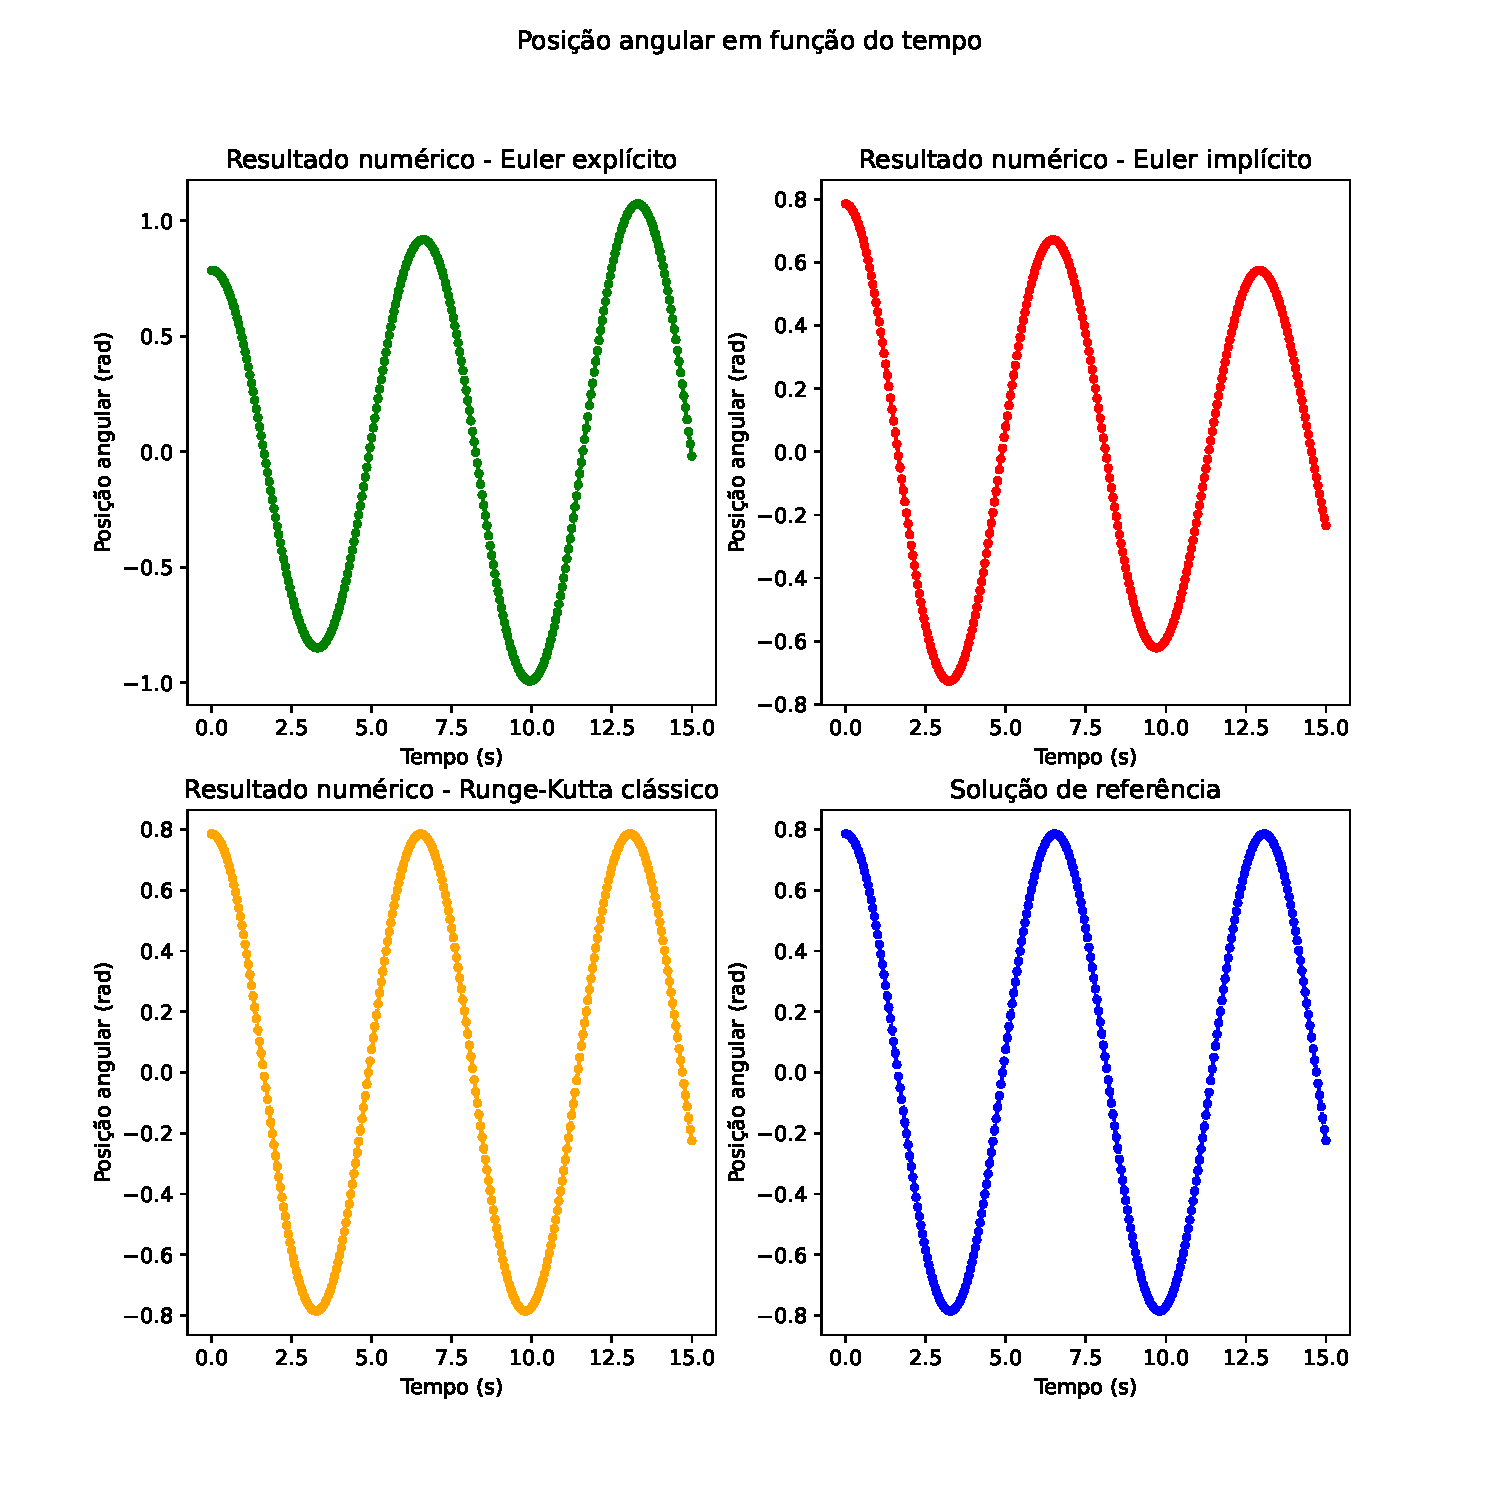
\includegraphics[width=\linewidth]{../images/p_posxtempo.pdf}
        \caption{Posição angular em função do tempo}\label{fig:t_x_rad}
    \end{figure}

    \subsubsection{Ordem de convergência}
    \begin{figure}[H]
        \centering
        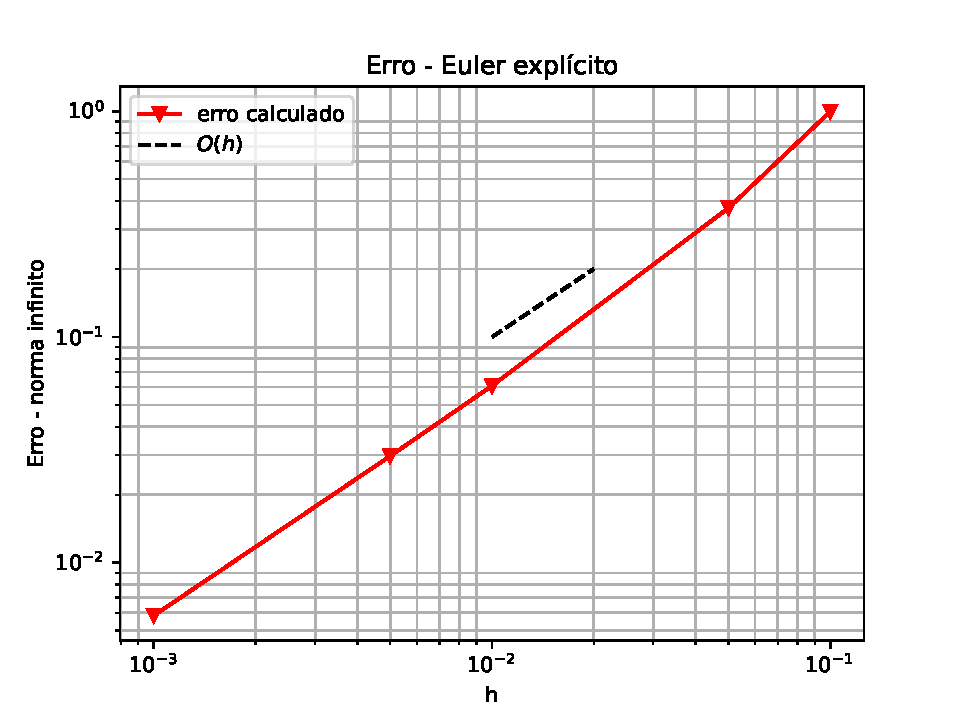
\includegraphics[width=0.45\linewidth]{../images/erro_explicito.pdf}
        \caption{Erro do método Euler Explícito}\label{fig:err_exp}
    \end{figure}

    \begin{figure}[H]
        \centering
        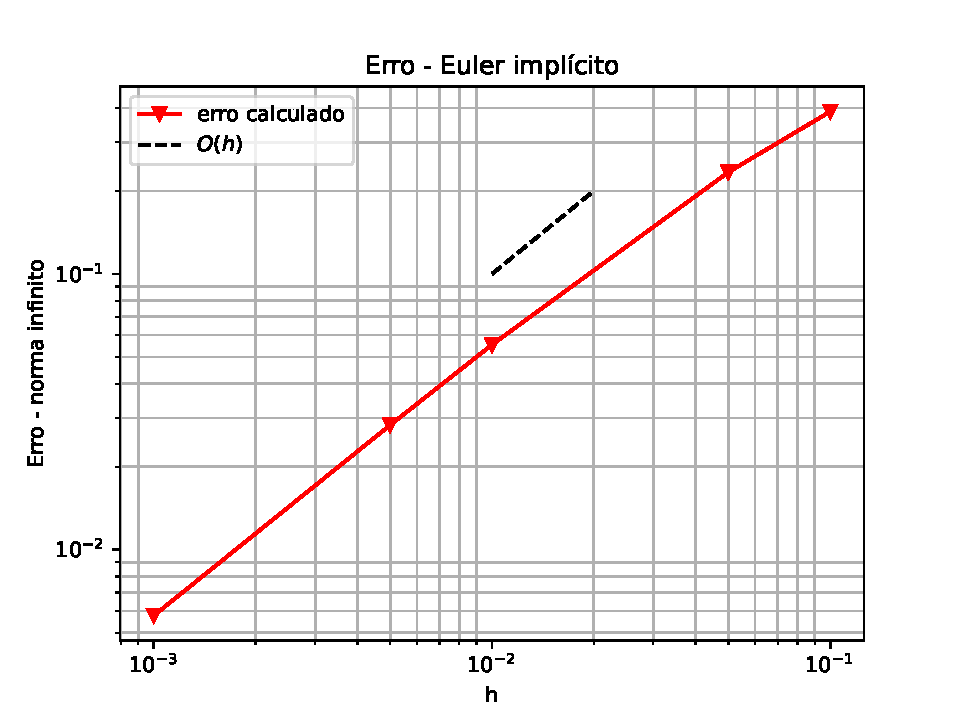
\includegraphics[width=0.45\linewidth]{../images/erro_implicito.pdf}
        \caption{Erro do método Euler Implícito}\label{fig:err_imp}
    \end{figure}

    \begin{figure}[H]
        \centering
        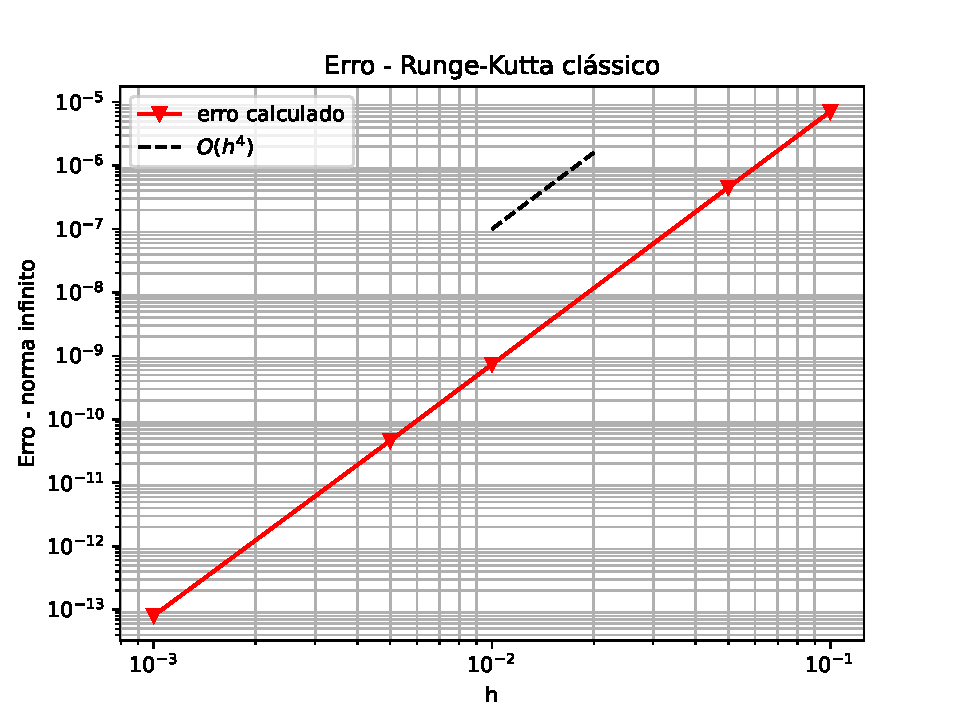
\includegraphics[width=0.45\linewidth]{../images/erro_RK4.pdf}
        \caption{Erro do método RK4}\label{fig:err_rk4}
    \end{figure}

    \subsubsection{Velocidade angular pela Posição angular}
    \begin{figure}[H]
        \centering
        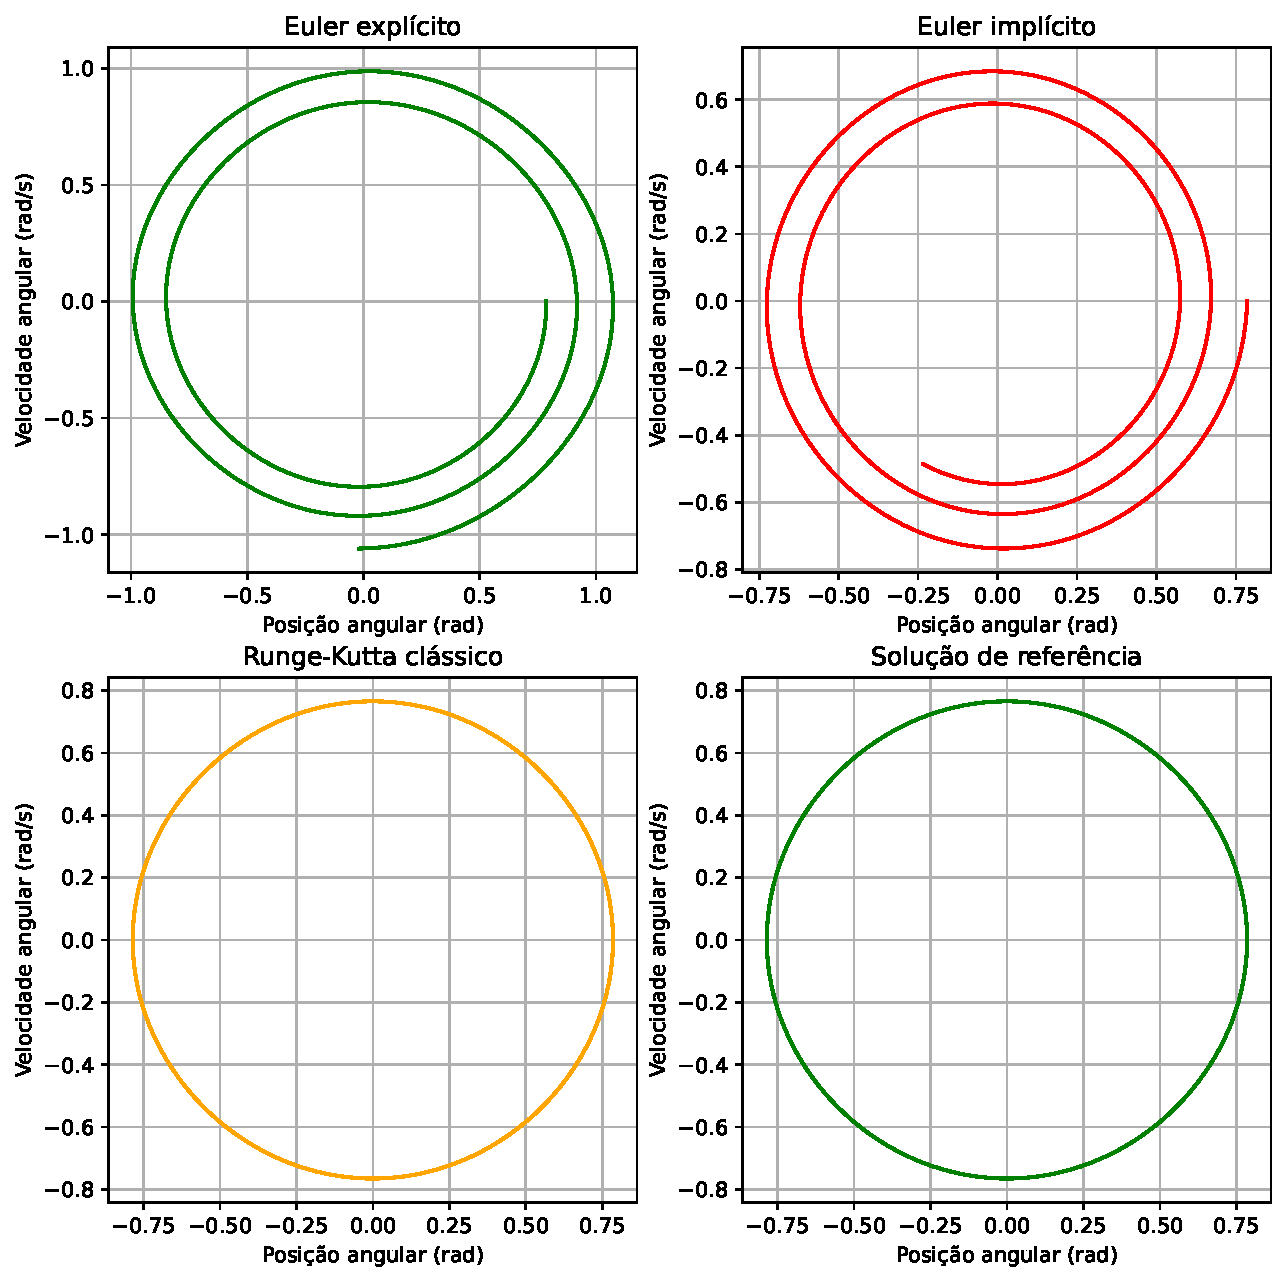
\includegraphics[width=\linewidth]{../images/retrato_fase.pdf}
        \caption{Velocidade angular em função da posição angular}\label{fig:rad_x_rad/s}
    \end{figure}

    % ---- %

    \section{Pêndulo Duplo}
    \subsection{EDO}
    \[\bd{u}(t) = \begin{pmatrix}
        u_1(t)\\
        u_2(t)\\
        u_3(t)\\
        u_4(t)\\
    \end{pmatrix} = \begin{pmatrix}
        q_1(t)\\
        q_2(t)\\
        p_1(t)\\
        p_2(t)
    \end{pmatrix}\]
    \[\bd{u}'(t) = \begin{pmatrix}
        q_1'(t)\\
        q_2'(t)\\
        p_1'(t)\\
        p_2'(t)
    \end{pmatrix} = \left.\begin{pmatrix}
        \frac{p_1-p_2\cos(q_1-q_2)}{2-\cos^2(q_1-q_2)}\\
        \frac{2p_2-p_1\cos(q_1-q_2)}{2-\cos^2(q_1-q_2)}\\
        -A_1+A_2-2\sin(q_1)\\
        A_1-A_2-\sin(q_2)
    \end{pmatrix}\right|_{(t)} = \left.\begin{pmatrix}
        \frac{u_3-u_4\cos(u_1-u_2)}{2-\cos^2(u_1-u_2)}\\
        \frac{2u_4-u_3\cos(u_1-u_2)}{2-\cos^2(u_1-u_2)}\\
        -A_1+A_2-2\sin(u_1)\\
        A_1-A_2-\sin(u_2)
    \end{pmatrix}\right|_{(t)} = \bd{f}(\bd{u}(t),t)\]
    onde
    \[A_1(t) = \left.\frac{p_1p_2\sin(q_1-q_2)}{1+\sin^2(q_1-q_2)}\right|_{(t)} = \left.\frac{u_3u_4\sin(u_1-u_2)}{1+\sin^2(u_1-u_2)}\right|_{(t)}\]
    \[A_2(t) = \left.\frac{[p_1^2+2p_2^2-2p_1p_2\cos(q_1-q_2)]\sin(q_1-q_2)\cos(q_1-q_2)}{[1+\sin^2(q_1-q_2)]^2}\right|_{(t)}\]
    \[= \left.\frac{[u_3^2+2u_4^2-2u_3u_4\cos(u_1-u_2)]\sin(u_1-u_2)\cos(u_1-u_2)}{[1+\sin^2(u_1-u_2)]^2}\right|_{(t)}\]

    \subsection{Trajetória de um pêndulo}
    \begin{figure}[H]
        \centering
        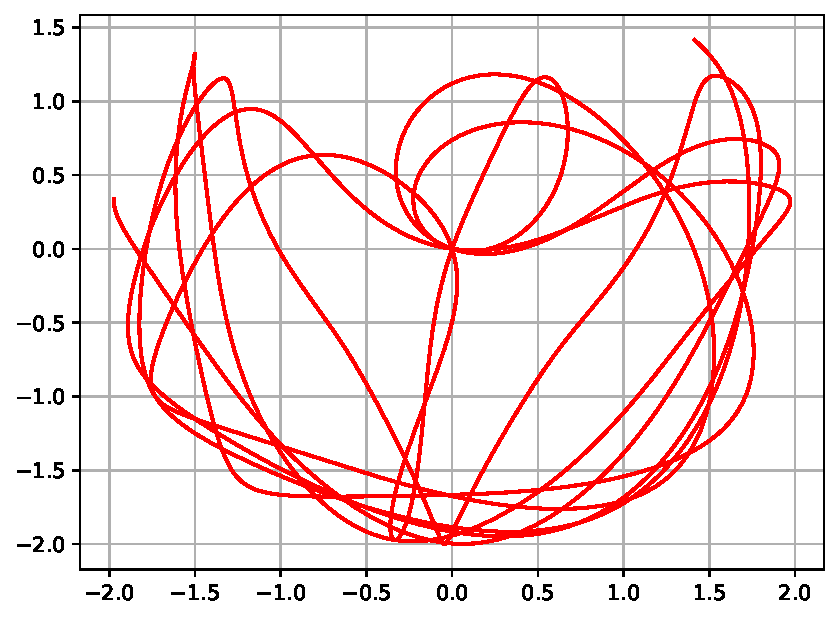
\includegraphics[width=0.5\linewidth]{../images/pendulo_duplo.pdf}
        \caption{Trajetória de um pêndulo, com $q_1(0)=q_2(0)=\dfrac{3\pi}{4}$}\label{fig:tra}
    \end{figure}

    \subsection{Experimentos}
    \begin{figure}[H]
        \centering
        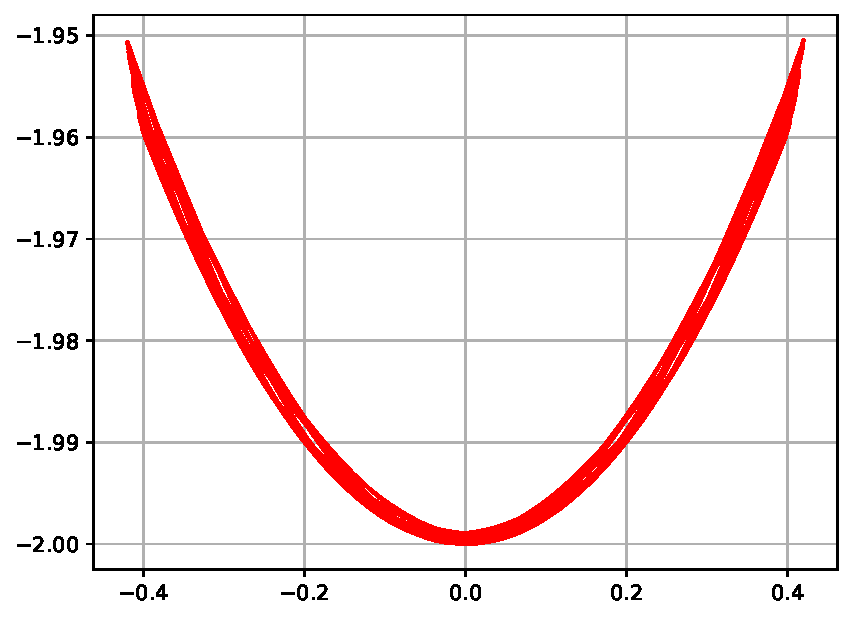
\includegraphics[width=0.5\linewidth]{../images/pendulo_duploeq.pdf}
        \caption{Experimento 1, com $q_1(0)=q_2(0)=0.2$}\label{fig:exp1}
    \end{figure}

    \begin{figure}[H]
        \centering
        \begin{subfigure}{0.48\textwidth}
            \centering
            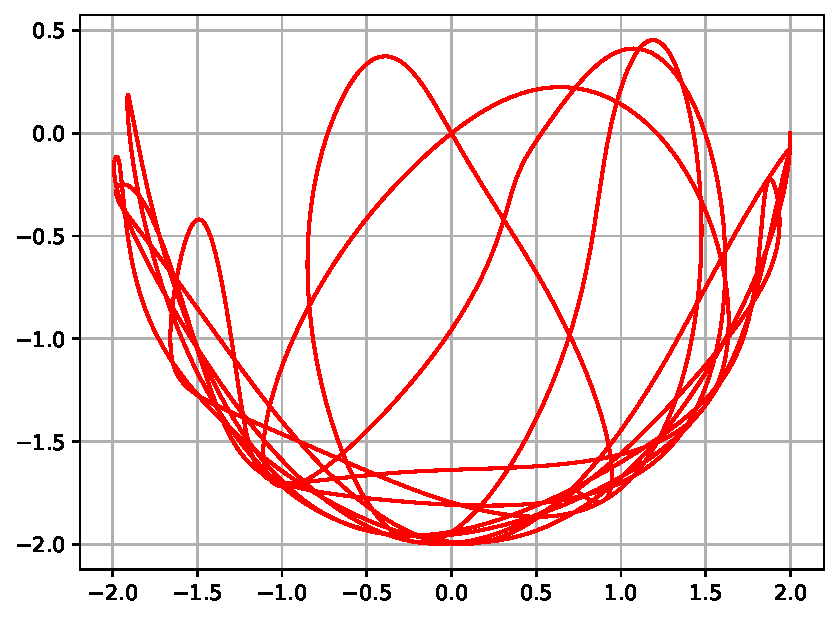
\includegraphics[width=\linewidth]{../images/pendulo_duplo1.pdf}
            \caption{Trajetória, com $q_1(0)=q_2(0)=\dfrac{\pi}{2}$}\label{fig:tra_1}
        \end{subfigure}\hfill
        \begin{subfigure}{0.48\textwidth}
            \centering
            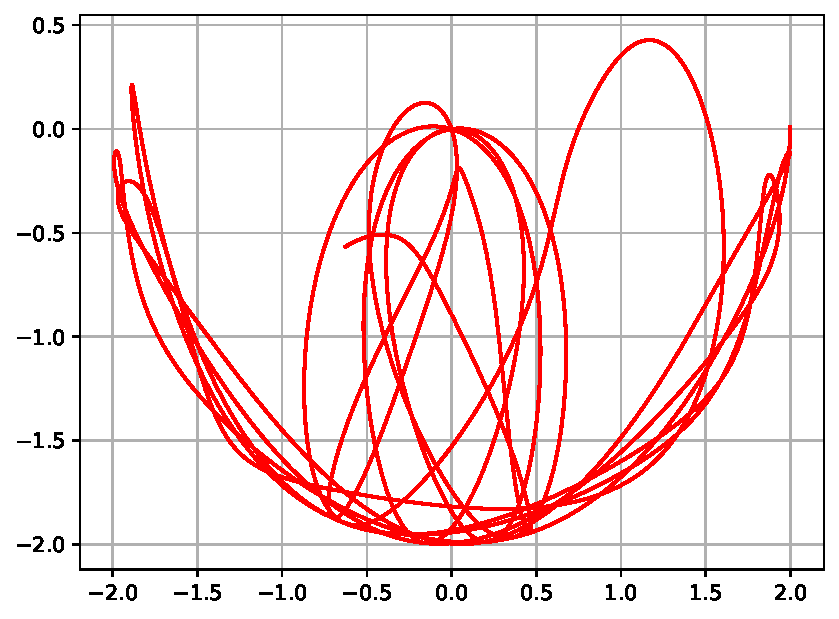
\includegraphics[width=\linewidth]{../images/pendulo_duplo2.pdf}
            \caption{Trajetória, com $q_1(0)=\dfrac{\pi}{2}$ e $q_2(0)=\dfrac{\pi}{2}+10^{-2}$}\label{fig:tra_2}
        \end{subfigure}
        \caption{Experimento 2}\label{fig:exp2}
    \end{figure}
\end{document}